	\documentclass[border = 12]{standalone}
	\usepackage{amsmath}
	\usepackage{stix}
	\usepackage{tikz}
	\usepackage{tkz-euclide}
	\usepackage{makecell}
	\usepackage{ifthen}
	\usepackage{pgfmath}
	\definecolor{blue}{RGB}{0,51,255} 
	\usetkzobj{all}
	
	\usetikzlibrary{intersections}
	\usetikzlibrary{decorations.markings}
	\usetikzlibrary{angles}
	\usetikzlibrary{quotes}
	\usetikzlibrary{calc}
	\usetikzlibrary{arrows}
	\usetikzlibrary{arrows.meta}
	\usetikzlibrary{shapes.geometric}
	\usetikzlibrary{patterns}
	\usetikzlibrary{shapes}
%For lines:
\definecolor{Grey}{RGB}{76,76,78}
\definecolor{Blue}{RGB}{85,164,224}
\definecolor{Red}{RGB}{225,75,59}
\definecolor{Green}{RGB}{16,158,36}
\definecolor{Orange}{RGB}{243,162,3}
\definecolor{Purple}{RGB}{124,36,231}
\definecolor{Fushia}{RGB}{225,50,162}



%For filling and shading:
\definecolor{Grey1}{RGB}{130,130,131}
\definecolor{Blue1}{RGB}{98,170,223}
\definecolor{Red1}{RGB}{236,98,88}
\definecolor{Green1}{RGB}{105,186,108}
\definecolor{Orange1}{RGB}{251,192,79}
\definecolor{Purple1}{RGB}{160,114,235}
\definecolor{Fushia1}{RGB}{237,97,174}

\usepackage{tikz-3dplot}
\usepackage{tikz}
\usetikzlibrary{calc,intersections,arrows.meta}
\begin{document}
	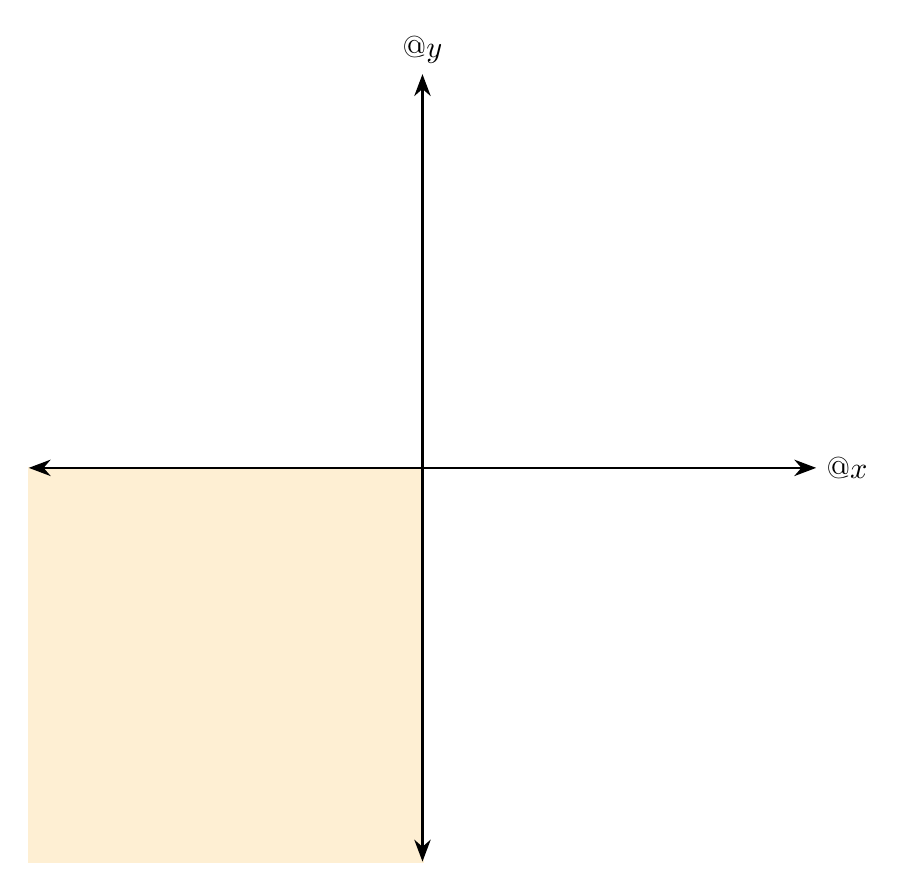
\begin{tikzpicture}
	

\begin{scope}[>={Stealth[scale=1.2]}, thick,font=\fontsize{11.25}{11.25}\selectfont]
\pgfgettransformentries{\mya}{\myb}{\myc}{\myd}{\mys}{\myt}
\pgfmathsetmacro{\preserve}{1/\mya}
\draw[Orange1!25,fill=Orange1!25] (0,0) rectangle +(-5,-5);
\draw [<->] (-5,0)--(5,0) node [anchor=west] {$@x$};
\draw [<->] (0,-5)--(0,5) node [anchor=south] {$@y$};

\end{scope}
		
		

		\end{tikzpicture}
	\end{document}
